% We have shown that Text2KB outperforms the baseline.
We now investigate how our system would compare to other systems on the same benchmark; then, we investigate in depth the different error modes (Section \ref{section:analysis:error}), which helps identify the areas of most substantial future improvements. 

We took an existing KBQA systems and demonstrated that by combining evidence from knowledge base and external text resources we can boost the performance.
A reasonable question is whether the same approach will be helpful to other systems, \eg the currently best system -- STAGG \cite{yih2015semantic}.
STAGG differs from our baseline system Aqqu in the components: entity linking algorithm, a set of query templates and ranking methods.
Therefore, our approach is complementary and should be helpful for STAGG as well.
To support this claim, we made an experiment to combine answers of STAGG and Text2KB.
One of the advantages of the former is its set of filters, that restricts list results to entities of certain type, gender, \etc
Therefore, we combined answers of STAGG and Text2KB using a simple heuristic: we chose to use the answer returned by STAGG if the number of answer entities is less than in the Text2KB answer, otherwise we use the answer of our approach.
Table \ref{table:combine_stagg} gives the results of the experiment, and as we can see the combination achieves a slightly better average F1 score.
Alternatively, we can look at the Oracle combination of the systems, which always selects the answer with the higher F1.
As we can see such a combination results in a performance of 0.606, which is much higher than either of the systems.

\begin{table}
\centering
\begin{tabular}{| p{4.5cm} | c | }
\hline
System  & F1 \\
\hline
%STAGG \cite{yih2015semantic} & 0.607 & 0.528 & 0.525\\
%Text2KB + STAGG & 0.598 & 0.534 & 0.532 (+1.3 \%) \\
%Text2KB + STAGG (Oracle) & 0.714 & 0.590 & 0.606 (+15.4 \%) \\
STAGG \cite{yih2015semantic} & 0.525\\
Text2KB + STAGG & 0.532 (+1.3 \%) \\
Text2KB + STAGG (Oracle) & 0.606 (+15.4 \%) \\
\hline
\end{tabular}
\vspace{-2mm}
\caption{Average F1 for combinations of Text2KB and STAGG using a simple heuristic based on the length of the answer list and Oracle upper bound}
\label{table:combine_stagg}
\vspace{-2mm}
\end{table}

As we mentioned earlier, answers to 112 of the test questions in the WebQuestions dataset involve predicates that weren't observed in the training set, which may be a problem for approaches that rely on a trained lexicon.
We evaluated both systems on these questions, and indeed the performance is very low, \ie the average F1 score of Text2KB is 0.1640 compared to 0.1199 for STAGG\footnote{Unfortunately, the number of questions is too low to show statistical significance (p-value=0.16) of the difference}.

\subsection{Error analysis}
\label{section:analysis:error}

\begin{figure}
\centering
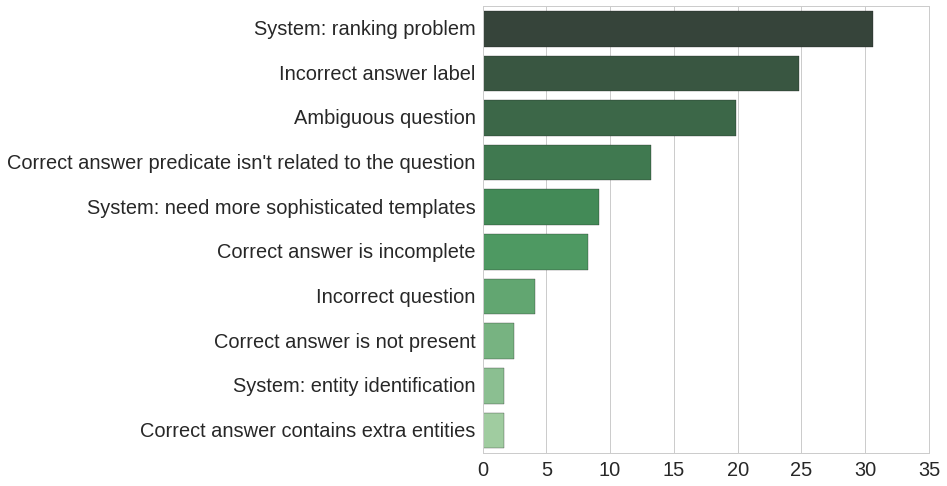
\includegraphics[width=0.4\textwidth]{img/error_analysis}
\vspace{-4mm}
\caption{Distribution of problems with questions, where Text2KB returns an answer with F1$<$1}
\label{fig:error_analysis}
\vspace{-2mm}
\end{figure}

To get a better insights into the problems that remain, we collected 1219 questions for which Text2KB didn't return completely correct answer, \ie F1 score $<$ 1.
We manually looked through a couple of hundreds of these examples and grouped the problems into several clusters (Figure \ref{fig:error_analysis}).

As we can see candidate ranking is still the major problem, and it accounts for $\sim31\%$ of the cases.
The second problem is incorrect ground truth labels (almost 25\% of reported errors).
Another set of questions has incomplete or overcomplete ground truth answer list.
Typical examples are questions asking for a list of movies, books, landmarks, \etc
The ground truth answer usually contains $\sim10$ entities, whereas the full list is often much larger.
This seems to be an artifact of the labeling process, where the answer was selected from the Freebase entity profile page, which shows only a sample of 10 entities, while the rest are hidden behind the ``N values total'' link.
About 20\% of the questions are ambiguous, \ie questions have no strict 1-1 correspondence with any of the predicates and can be answered by multiple ones without any obvious preferences.
For example, the question \textit{``what did hayes do?''} can be answered by profession, occupied position or some other achievements.
Another problem is when there is no predicate that answers the question.
For example, the question \textit{``what do people in france like to do for fun?''} doesn't have a good match among the facts stored in Freebase.
The ground truth entity \texttt{Cycling} comes from the list Olympic sport competitions country participated\footnote{\texttt{olympics.olympic\_participating\_country.athletes}}.

Text2KB components were quite effective in resolving some of the problems.
Web search results helped identify the right question topical entity in a number of cases, \eg \textit{``what did romo do?''} mentions only the last name of the Dallas Cowboys quarterback and the baseline system were unable to map it to the right entity.
Web search results provides more than enough evidence that ``\textit{romo}'' refers to \texttt{Tony Romo}.
However, there are a number of loses, introduced by added unrelated entities.
For example, the entity \texttt{I Love Lucy} was added for the question \textit{``what was lucille ball?''}, because the term \textit{lucy} had high similarity with \textit{lucille}.
A portion of these problems can be fixed by a better entity linking strategy, \eg \cite{SMAPH_ERD:2014}.
An interesting example, when external text resources improved the performance is the question \textit{``what ship did darwin sail around the world?''}.
This is actually a hard question, because the ship entity is connected to the \texttt{Charles Darwin} entity through the ``knownFor'' predicate along with some other entities like \texttt{Natural selection}.
% \footnote{\texttt{user.lindenb.default\_domain.scientist.known\_for}
Thus, the predicate itself isn't related to the question, but nevertheless, the name of the ship \texttt{HMS Beagle} is mentioned multiple times in the web search results, and entity pair model computed from ClueWeb also has high scores for the terms ``ship'' and ``world''.

There are several major reasons for the loses, introduced by features based on external text resources.
Some entities often mentioned together and therefore one of them gets high values of cooccurrence features.
For example, the baseline system answered the question \textit{``when did tony romo got drafted?''} correctly, but since \texttt{Tony Romo} is often followed by \texttt{Dallas Cowboys}, Text2KB ranked the team name higher.
Another common problem with our features is an artifact of entity linking, which works better for names and often skips abstract entities, like professions.
For example, the correct answer to the question \textit{``what did jesse owens won?''} is an entity with the name \texttt{Associated Press Male Athlete of the Year}, which is rarely mentioned or it's hard to find such mentions.
Some problems were introduced by a combination of components.
For example, for \textit{``where buddha come from?''} a topical entity \texttt{Buddhism} was introduced from search results, and it generated \texttt{Gautama Buddha} as one of the answer candidates.
This answer was ranked the highest due to large number of mentions in the search results.

In summary, we show that ideas behind Text2KB could be integrated into other systems and improve their performance.
The error analysis suggested that even though a significant number of questions in the WebQuestions dataset have incorrect or ambiguous ground truth labels, there is still a room for improvement.
In particular, the future work for Text2KB will include a better strategy for entity linking using external data sources and a better context model for entity mentions in text documents, which can put more weight on entities mentioned in the context related to the question.
